%%%%%%%%%%%%%%%%%%%%%%%%%%%%%%%%%%%%%%%%%%%%%%%%%%%%%%%%%%%%%%%%%%%%%%%%%%%%%%%
% Definici�n del tipo de documento.                                           %
% Posibles tipos de papel: a4paper, letterpaper, legalpapper                  %
% Posibles tama�os de letra: 10pt, 11pt, 12pt                                 %
% Posibles clases de documentos: article, report, book, slides                %
%%%%%%%%%%%%%%%%%%%%%%%%%%%%%%%%%%%%%%%%%%%%%%%%%%%%%%%%%%%%%%%%%%%%%%%%%%%%%%%
\documentclass[a4paper,10pt]{article}
\usepackage[paperwidth=190mm,paperheight=290mm,left=1.5cm,top=3cm,right=1.5cm,bottom=1cm,head=2.0cm,includefoot]{geometry}

%%%%%%%%%%%%%%%%%%%%%%%%%%%%%%%%%%%%%%%%%%%%%%%%%%%%%%%%%%%%%%%%%%%%%%%%%%%%%%%
% Los paquetes permiten ampliar las capacidades de LaTeX.                     %
%%%%%%%%%%%%%%%%%%%%%%%%%%%%%%%%%%%%%%%%%%%%%%%%%%%%%%%%%%%%%%%%%%%%%%%%%%%%%%%

% Paquete para inclusi�n de gr�ficos.
\usepackage{graphicx}
\usepackage{multirow}
\usepackage{bigstrut}
\usepackage{lastpage}
\usepackage{fancyhdr}
\usepackage{pdfpages}
\usepackage[pdfborder={0 0 0}]{hyperref}


\renewcommand{\headrulewidth}{1pt}
\renewcommand{\footrulewidth}{1pt}
\usepackage{setspace}
% Paquete para definir la codificaci�n del conjunto de caracteres usado
% (latin1 es ISO 8859-1).
\usepackage[latin1]{inputenc}

% Paquete para definir el idioma usado.
\usepackage[spanish]{babel}

\pagestyle{fancy}
\lhead{Trabajo pr�ctico 1}
\cfoot{P�gina \thepage~de \pageref{LastPage}}
\rfoot{$2^{do}$ Cuatrimentre 2016}

% T�tulo principal del documento.
\title{		\textbf{Trabajo pr�ctico 1: conjunto de instrucciones MIPS}}

% Informaci�n sobre los autores.
\author{	Tomas Franco, \textit{Padr�n Nro. 00.000}                     \\
            \texttt{ direcci�n de e-mail }                                              \\
            Diego Meler, \textit{Padr�n Nro. 91.299}                     \\
            \texttt{ dmeller@fi.uba.ar }                                              \\[2.5ex]
            \normalsize{Grupo Nro.  - 2do. Cuatrimestre de 2016}                       \\
            \normalsize{66.20 Organizaci�n de Computadoras}                             \\
            \normalsize{Facultad de Ingenier�a, Universidad de Buenos Aires}            \\
       }
\date{}



\begin{document}

% Inserta el t�tulo.
\maketitle

% Quita el n�mero en la primer p�gina.
\thispagestyle{empty}

% Resumen
\begin{abstract}
Realizamos el Juego de la Vida de Conway descripto en el enunciado, realizamos un Makefile para diferenciar las compilaciones con la funci�n de vecinos en C y en MIPS32, elegimos como modelo de universo Toroidal y los archivos de salida fueron realizados en el formato Plain PBM
\end{abstract}

\newpage

\section{Enunciado}

\begin{figure}
   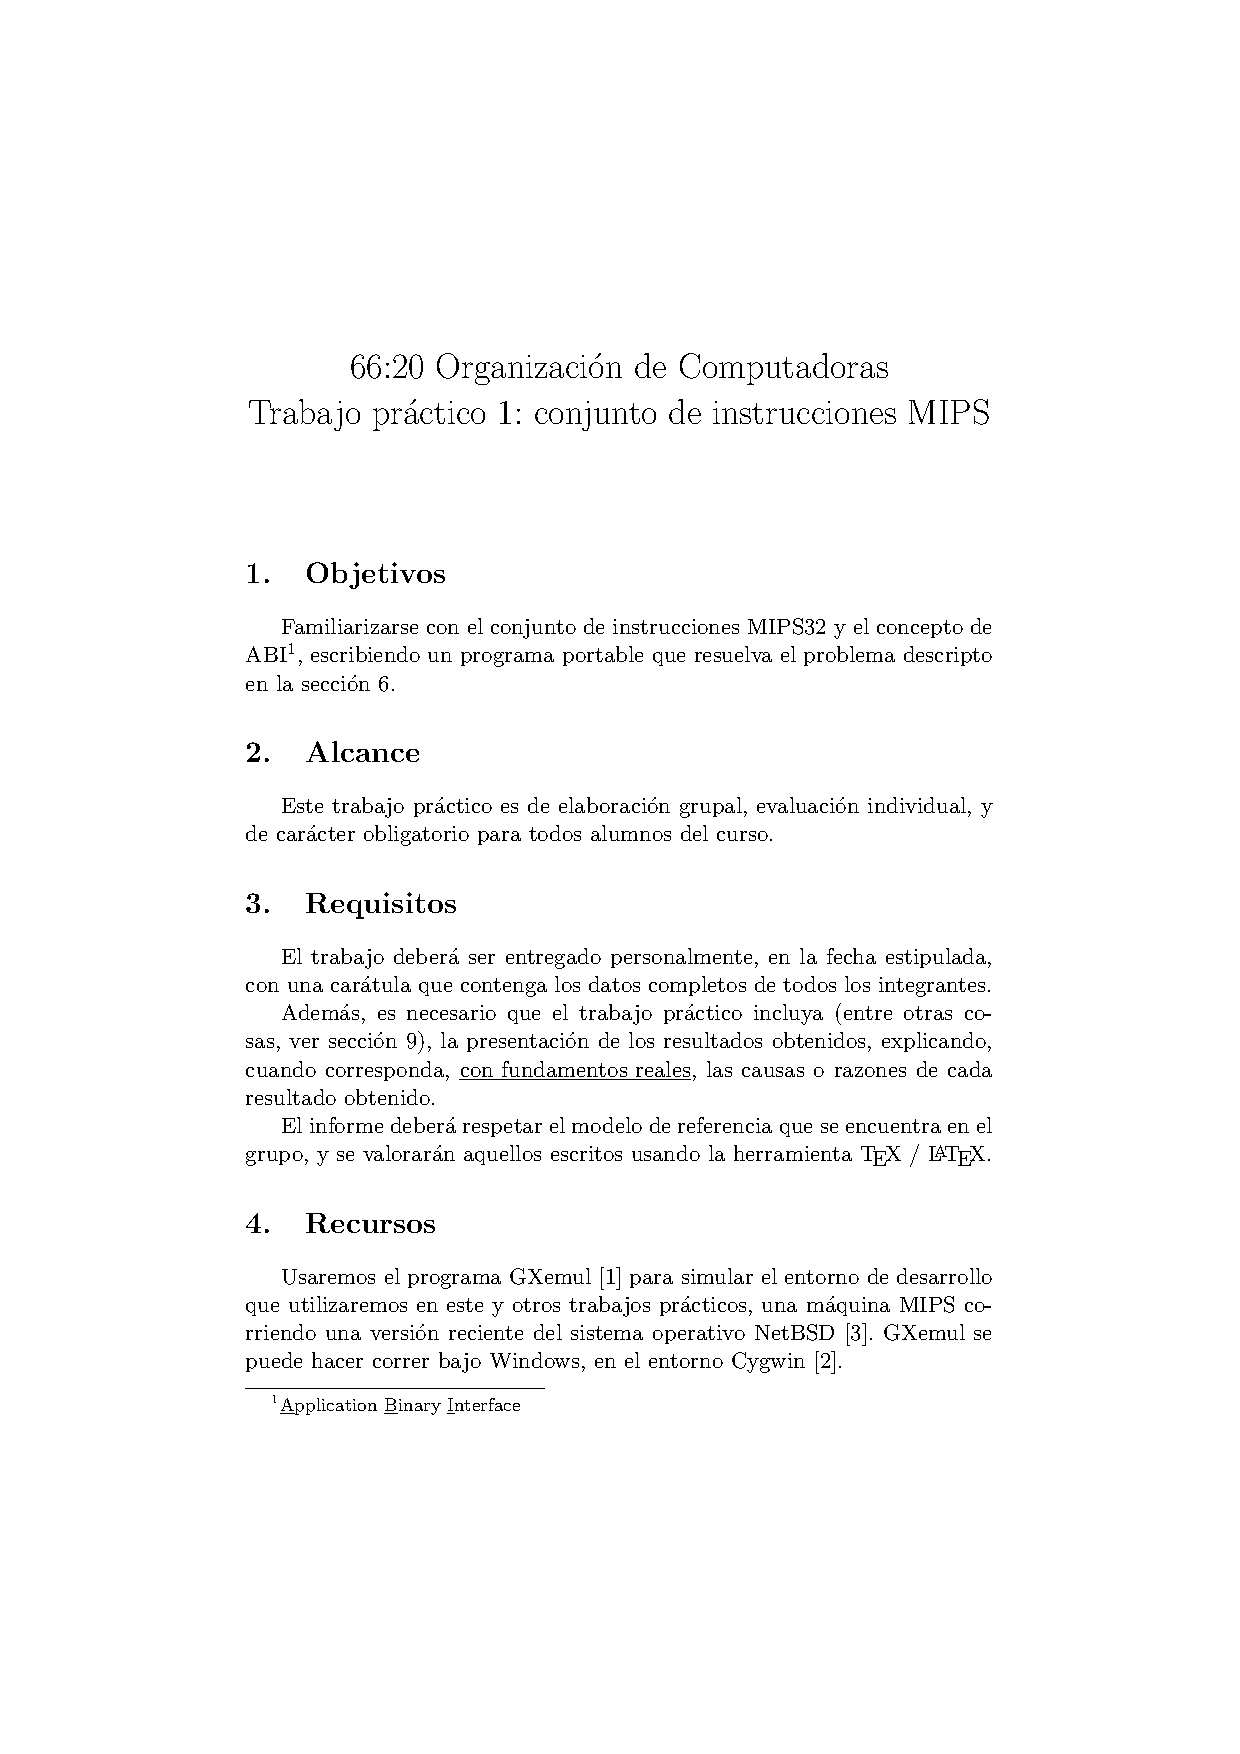
\includepdf[pages={1},nup=1x1]{tp1-c2-2016.pdf}      
 \label{fig:Test}
\end{figure}

\includepdfset{pages={2-},nup=1x1,landscape=false}
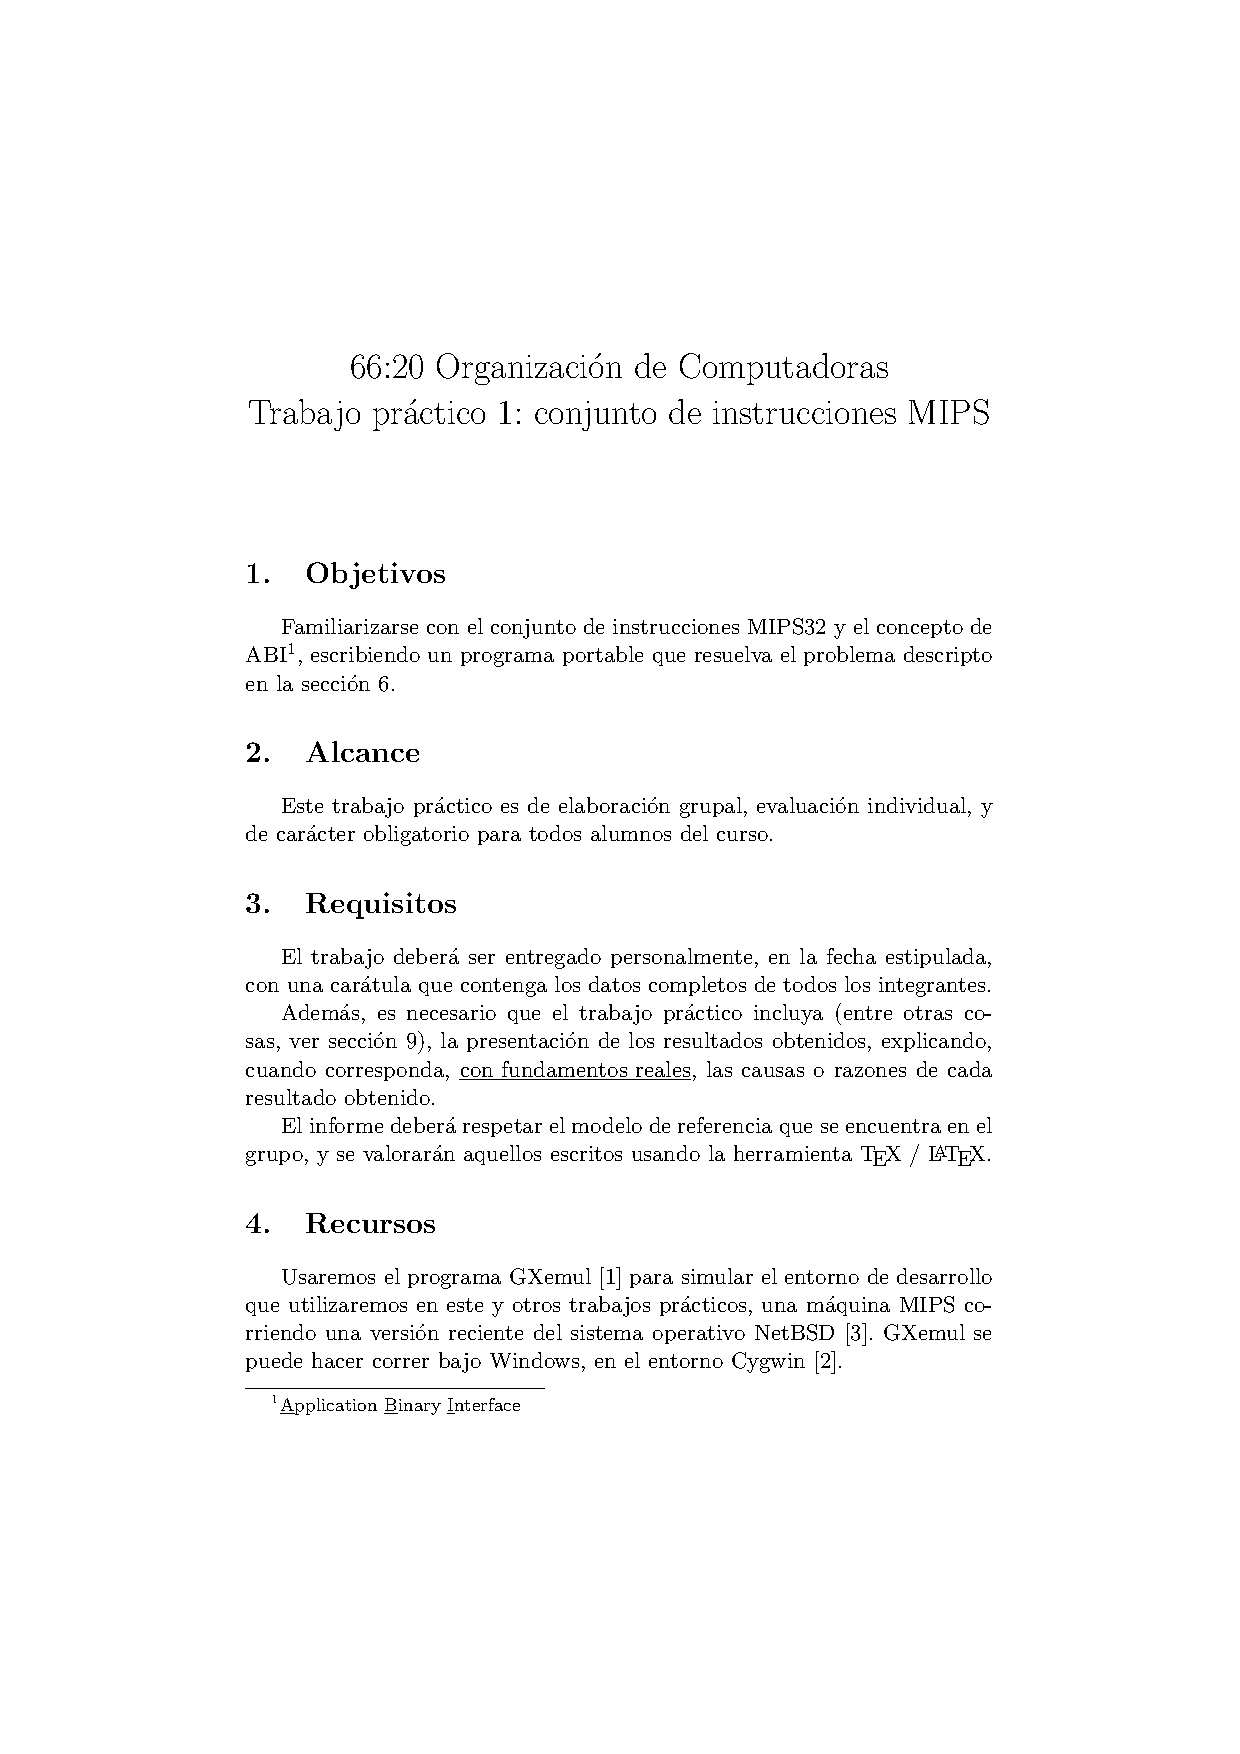
\includepdf[scale=0.85, pagecommand={\thispagestyle{fancy}}]{tp1-c2-2016.pdf}

\section{Dise�o e Implementaci�n del programa}

\subsection{Dise�o}
En la tabla~\ref{tab001} se muestra un ejemplo de c�mo se insertan las mismas en un documento \TeX{} / \LaTeX{}.

\subsection{Implementaci�n}


\subsection{Funci�n Vecinos}

\subsubsection{Stack para la ABI}
\begin{center}
\begin{tabular}{|c|c|c|}
\hline
ABI & Tama�o & Guarda \\
\hline
\multirow{2}{*}{SRA} & \multirow{2}{*}{8} & fp \\\cline{3-3}
& & gp \\
\hline
\multirow{2}{*}{LTA} & \multirow{2}{*}{8} & PADDING \\\cline{3-3}
& & V \\
\hline
\end{tabular}
\end{center}

El total del stack a reservar es de 16 Mb

\subsubsection{Par�metros de la funci�n}
Sabemos que en las posiciones 16,20,24,28 y 32 tenemos los 5 par�metros de la funci�n

\begin{center}
\begin{tabular}{|c|c|}
\hline
Posici�n & Guarda \\
\hline
32 & N \\
\hline
28 & M \\
\hline
24 & J \\
\hline
20 & I \\
\hline
16 & A \\
\hline
0 & ABI \\
\hline
\end{tabular}
\end{center}

\section{Corridas de prueba}

\subsection{Glider}
\begin{center}


\begin{tabular}{ c | c }


\includegraphics[scale=0.25]{glider_0.png}  & 
\includegraphics[scale=0.25]{glider_1.png}  \\
glider\_0.pbm	& glider\_1.pbm \\

\includegraphics[scale=0.25]{glider_2.png}  & 
\includegraphics[scale=0.25]{glider_3.png}  \\
glider\_2.pbm	& glider\_3.pbm \\

\includegraphics[scale=0.25]{glider_4.png}  & 
\includegraphics[scale=0.25]{glider_5.png}  \\
glider\_4.pbm	& glider\_5.pbm \\

\includegraphics[scale=0.25]{glider_6.png}  & 
\includegraphics[scale=0.25]{glider_7.png}  \\
glider\_6.pbm	& glider\_7.pbm \\

\includegraphics[scale=0.25]{glider_8.png}  & 
\includegraphics[scale=0.25]{glider_9.png}  \\
glider\_8.pbm	& glider\_9.pbm \\

\includegraphics[scale=0.25]{glider_10.png}  & \\
glider\_10.pbm	&  \\
\end{tabular}
\end{center}


\subsection{Pento}


\subsection{Sapo}


% Inclusi�n de una imagen en formato EPS (Encapsulated Postscript).
\begin{figure}[!htp]
\begin{center}
%\includegraphics[width=0.5\textwidth]{fig001.eps}
\end{center}
\caption{Facultad de Ingenier�a $-$ Universidad de Buenos Aires.} \label{fig001}
\end{figure}

\section{C�digo Fuente}

\includepdfset{pages=-,nup=1x2,landscape=true} 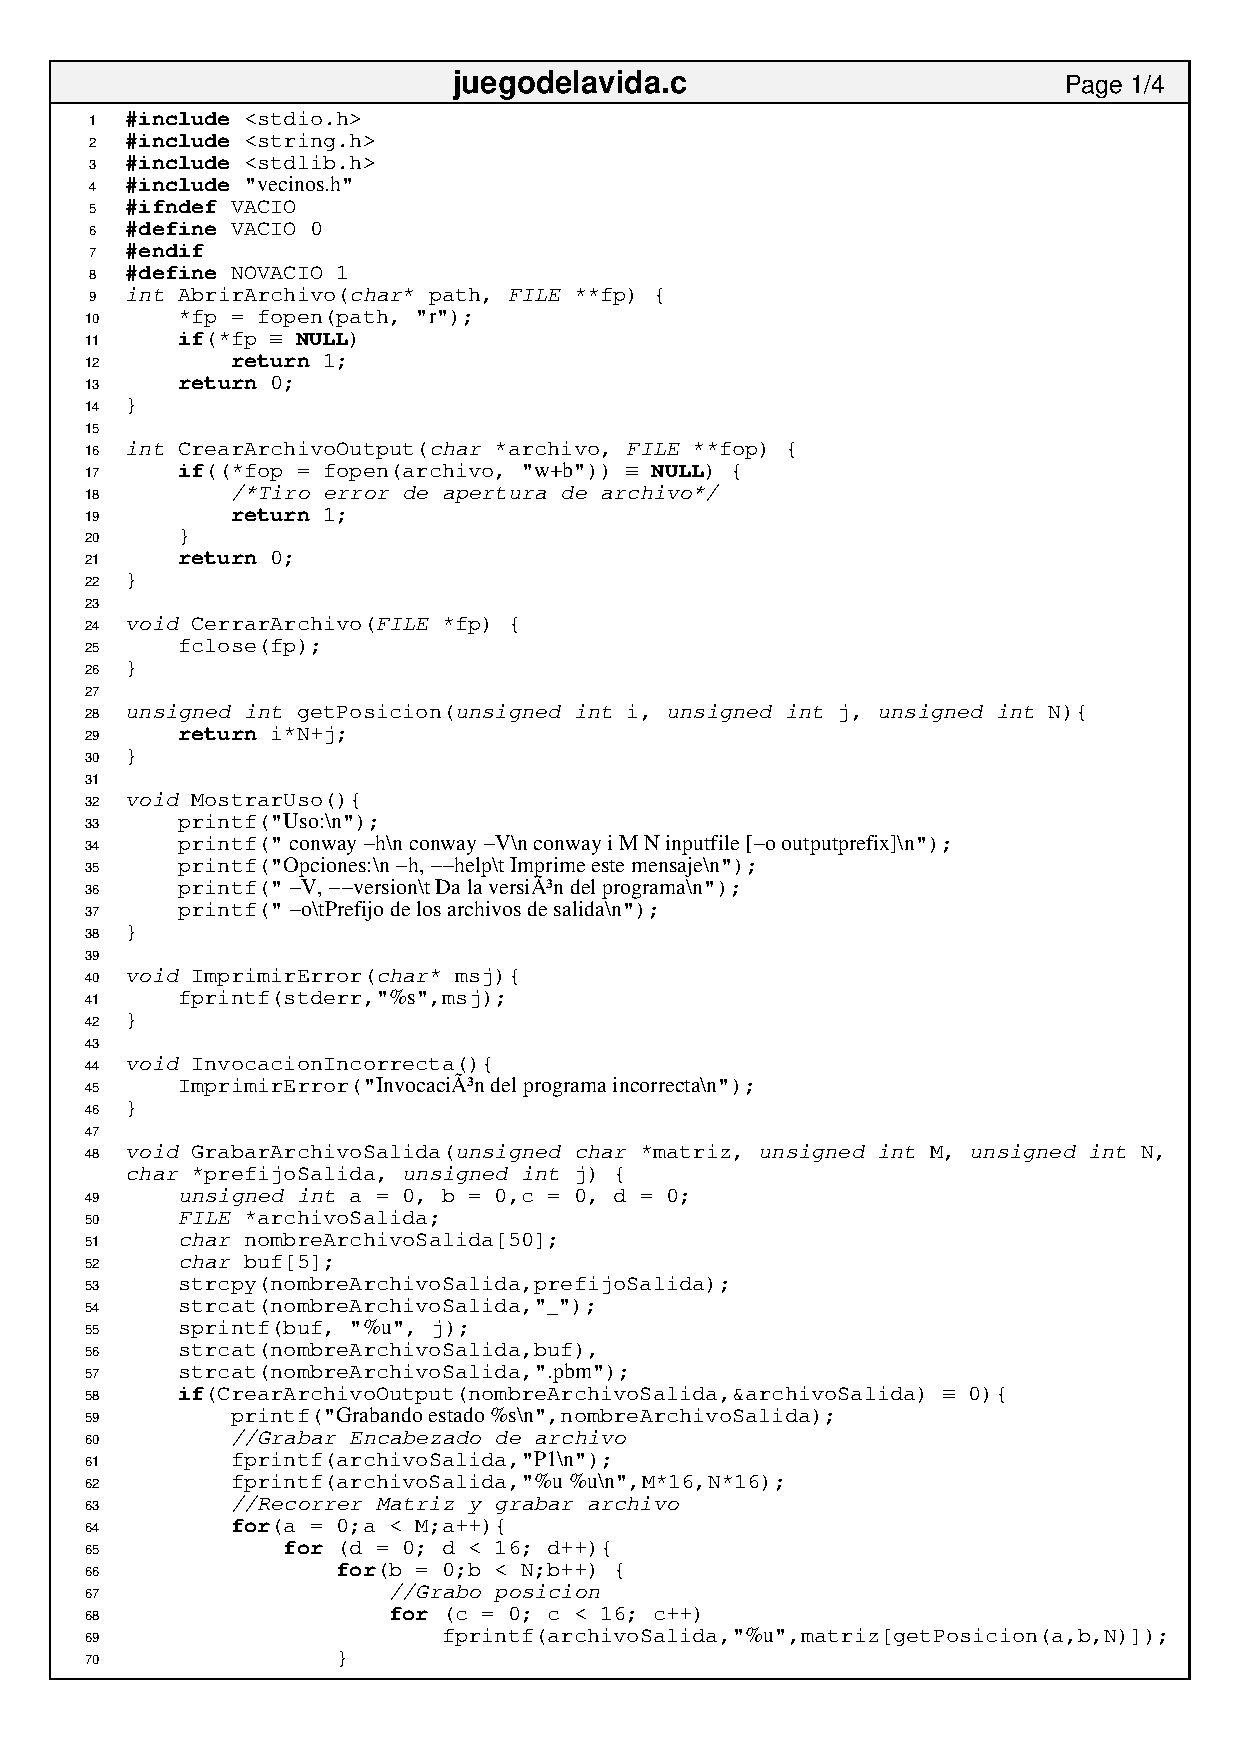
\includepdf[scale=0.85, pagecommand={\thispagestyle{fancy}}]{codigo.pdf}

\section{Conclusiones}

Se present� un modelo para que los alumnos puedan tomar como referencia en la redacci�n de sus informes de trabajos pr�cticos.


% Citas bibliogr�ficas.
\begin{thebibliography}{99}

\end{thebibliography}

\end{document}
